
\documentclass[11pt,a4paper]{report}

% Packages
% Paquetes para tildes
\usepackage[utf8]{inputenc}
\usepackage[spanish, es-tabla]{babel}
\usepackage{caption}
\addto\captionsspanish{
\renewcommand{\chaptername}{Práctica}
}

\usepackage{titlesec}
\usepackage{listings}
\usepackage{adjustbox}
\usepackage{enumitem}
\usepackage{boldline}
\usepackage{amssymb, amsmath}
\usepackage[margin=1in]{geometry}
\usepackage{xcolor}
\usepackage{soul}
\usepackage{amsthm}
%Paquete para imágenes
\usepackage{graphicx,wrapfig,lipsum}
%Paquete para hiperlinks
\usepackage[hidelinks]{hyperref}
%Paquetes para códigos
\usepackage{listings}
\usepackage{color}

\definecolor{dkgreen}{rgb}{0,0.6,0}
\definecolor{gray}{rgb}{0.5,0.5,0.5}
\definecolor{mauve}{rgb}{0.80,0.40,0.0}

\lstset{frame=tb,
  language=Python,
  aboveskip=3mm,
  belowskip=3mm,
  showstringspaces=false,
  columns=flexible,
  basicstyle={\small\ttfamily},
  numbers=none,
  numberstyle=\tiny\color{gray},
  keywordstyle=\color{blue},
  commentstyle=\color{dkgreen},
  stringstyle=\color{mauve},
  breaklines=true,
  breakatwhitespace=true,
  tabsize=3
}
%%%%%%%%%%Fin de configuración para códigos%%%%%%%


%%%%%%%%%%		Tabular		%%%%%%%%%%%
\newcommand\tab[1][1cm]{\hspace*{#1}}
%%%%%%%%%%		Tabular		%%%%%%%%%%%


\titleformat{\chapter}[display]{\normalfont\bfseries}{}{0pt}{\Huge}

\usepackage{graphicx}
\usepackage{amsmath}
\begin{document}
\begin{titlepage}
  \centering

  \vspace{10cm}

                  {\scshape\Huge \textbf{APRENDIZAJE AUTOMÁTICO} \par} \vspace{1cm}
                  \vspace{5.0cm}
                         {\large\huge PRÁCTICAS - PRÁCTICA 0\\}
                         \vspace{1.7cm}
                                {\large{\huge{\scshape Pedro Gallego López}}\vspace{1.30cm}\\ \LARGE \scshape Doble Grado de Ingeniería Informática y Matemáticas \par} \vspace{8.0cm}
                                {\large\itshape Universidad de Granada \\ Escuela Técnica Superior de Ingeniería Informática y Telecomunicaciones \par} \vspace{1.00cm}
                                

                                \vfill
                                % Bottom of the page
                                    {\large \today\par}

\end{titlepage}

\newpage

\chapter{Práctica 0}
\section*{Introducción}
La práctica en cuestion se propone para reforzar los conocimientos adquiridos en las primeras clases de rácticas, en donde se han introducido los principios de \emph{Python}, \emph{Matplotlib}, \emph{Numpy} y \emph{Scikit-learn}.

\section*{Ejercicio 1}
\subsubsection{Leer la base de datos de iris que hay en scikit-learn. Obtener las características (datos de entrada X) y la clase (y). Quedarse con las características 1 y 3 (primera y tercera columna de X). Visualizar con un color diferente (con naranja, negro y verde), e indicando con una leyenda la clase a la que corresponde cada color}

La base de datos \textbf{iris} contiene 3 tipos de flores iris: Setosa, Versicolor y Virginica, donde se tienen sus cuatro características: ancho y alto del sépalo además del ancho y largo del pétalo. Esto guardado en un \texttt{numpy.ndarray} de $150\times4$.\\

Para poder cargar la base de datos iris hacemos uso de los datasets de \texttt{sklearn}: utilizamos concretamente \texttt{datasets.load\_iris()}. Lo guardamos en una variable denominada \texttt{iris}, esta variable contiene dos atributos que nos darán precisamente las características y la clase, estos atributos son \texttt{iris.data} y \texttt{iris.target} respectivamente. Para quedarnos con las características 1 y 3, que son el largo tanto del sépalo como del pétalo, hacemos uso del acceso a los elementos del array que proporciona numpy: \texttt{array[:,:3:2]} cogiendo las filas pares menores menores que 3, así serían la 0 y la 2, que justamente son las características que nos piden.
\begin{itemize}
\item \texttt{X = iris.data[:,:3:2]}
\item \texttt{y = iris.target}
\end{itemize} 
Para los colores he cogido los siguientes en formato hexadecimal:
\begin{itemize}
\item Naranja: \#FF9300
\item Negro: \#000000
\item Verde: \#31BF00
\end{itemize}
La asignación de estos colores la hacemos dentro de la función \texttt{plt.scatter} donde al parámetro \texttt{cmap} le asignamos \texttt{colors.ListedColormap(colores)} siendo \texttt{colores} un vector que contiene los colores nombrados anteriormente. Al parámetro \texttt{edgecolor} le asignamos el valor \texttt{`k'} para que tengan borde los puntos y podamos diferenciarlos. Asignamos también nombre a los ejes.\\

Para la leyenda debemos de coger la salida que nos da \texttt{plt.scatter} y coger como parámetro \texttt{handle} de la función \texttt{plt.legend}: \texttt{scatter.legend\_elements()[0]} para saber a qué punto asignar cada etiqueta. Las etiquetas las cogemos directamente de nuestra variable \texttt{iris}\\

El resultado sería el siguiente:
\begin{figure}[htp]
\centering
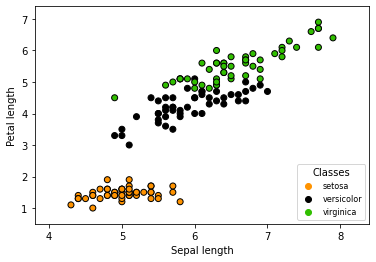
\includegraphics[scale=1.00]{imagenes/Ejercicio1.png}
\caption{}
\label{t2}
\end{figure}




\section*{Ejercicio 2}
\subsection*{Separar en training (75 \% de los datos) y test (25 \%) aleatoriamente conservando la proporción de elementos en cada clase tanto en training como en test. Con esto se pretende evitar que haya clases
infra-representadas en entrenamiento o test.}
\texttt{train\_test\_split} de \texttt{sklearn.model\_selection} va a ser la función que nos va a solucionar el ejercicio. Cargamos los datos en \texttt{(X,y)} y ejecutamos la línea:

\begin{itemize}
\item \texttt{X\_train, X\_test, y\_train, y\_test = train\_test\_split(X, y, train\_size=0.75,}\\ \tab\tab\tab\tab\tab\tab\tab\tab\tab\tab \texttt{ shuffle=True, stratify=y)}
\end{itemize}

Donde hemos definido en \texttt{train\_size=0.75} que el training tenga el 75\% de los datos y el test el 25\%. Con \texttt{shuffle=True} damos aleatoriedad y con \texttt{stratify=y} conseguimos mantener la proporción que nos pide el enunciado. Para comprobar que de verdad se cumple esto he hecho comprobaciones con print, la salida está en la tabla 1.1.

Vemos como en el caso del TEST no es exactamente 1/3 del total y dista un poco, esto se debe a que el número $0.25\times150$ que es el número de test que hay, no es un número entero, esto hará que el reparto no sea exactamente igual, pero si lo más aproximado posible. Es más, ejecutando varias veces el código se observa como las proporciones son exactamente las mismas permutándose entre ellas.

\begin{table}[htb]

\centering
\begin{tabular}{|l|}

\hline
	Cantidad del train: 112 que supone un 0.7466666666666667\% del total\\
Cantidad del test: 38 que supone un 0.25333333333333335\% del total\\
En el TOTAL están las proporciones\\
   \tab Clase 1: 0.3333333333333333\%\\
   \tab Clase 2: 0.3333333333333333\%\\
   \tab Clase 3: 0.3333333333333333\%\\
En el TRAIN están ahora las proporciones\\
   \tab Clase 1: 0.33035714285714285\%\\
   \tab Clase 2: 0.33035714285714285\%\\
   \tab Clase 3: 0.3392857142857143\%\\
En el TEST están ahora las proporciones\\
   \tab Clase 1: 0.34210526315789475\%\\
   \tab Clase 2: 0.34210526315789475\%\\
   \tab Clase 3: 0.3157894736842105\%\\
\hline
\end{tabular}
\label{t:salida}
\caption{Salida de comprobación de resultados}
\end{table}

\section*{Ejercicio 3}
\subsection*{Obtener 100 valores equiespaciados entre 0 y 4$\pi$. Obtener el valor de sin(x), cos(x) y tanh(sin(x)+cos(x)) para los 100 valores anteriormente calculados. Visualizar las tres curvas simultáneamente en el mismo plot (con líneas discontinuas en verde, negro y rojo).}
Para obtener los 100 valores equiespaciados entre 0 y 4$\pi$ usamos 
\begin{itemize}
\item \texttt{np.linspace(0, 4*np.pi, (100))}
\end{itemize}

Obtenemos los valores de las funciones con \texttt{y1=np.sin(x)}, \texttt{y2=np.cos(x)} y \texttt{y3=np.tanh(y1+y2)} aprovechando los valores ya calculados con \texttt{y1, y2}. Creamos los plots con \texttt{plt.subplots()} y utilizamos los parámetros \texttt{`g--',`k--',`r--'} para conseguir las líneas discontinuas en verde, negro y rojo: las letras marcan el color y el \texttt{--} marca que sea discontinua. El resultado sería el siguiente:
\begin{figure}[htp]
\centering
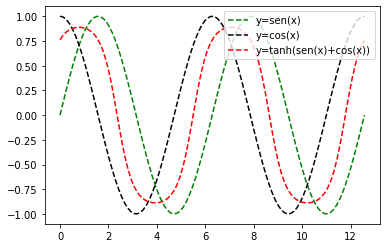
\includegraphics[scale=0.90]{imagenes/Ejercicio3.png}
\caption{Gráfica del ejercicio 3.}
\label{t3}
\end{figure}












\end{document}


















